% Sección 2: Datos hospitalarios y reconstrucción del flujo asistencial
% evidencia:E03,E06,E07,E19

\section{Datos hospitalarios y reconstrucción del flujo asistencial}

El análisis parte del repositorio PostgreSQL de solo lectura alojado en el esquema institucional compatible con OMOP CDM v5.4 \parencite{ohdsi54,mediflow2026inventario}. En concordancia con el principio de privacidad del certamen y con las decisiones iniciales del equipo, ninguna etapa del flujo analítico descarga filas individuales de pacientes ni identificadores clínicos: todas las extracciones se ejecutan en origen mediante 24 consultas SQL agregadas que exportan únicamente conteos por hora, día, mes o concepto hacia almacenamiento local protegido fuera del control de versiones \parencite{mediflow2026informe,mediflow2026auditoria}.

\subsection{Esquema OMOP disponible frente a uso efectivo y cortes temporales}

Una distinción metodológica indispensable separa las tablas visibles en el catálogo OMOP del subconjunto efectivamente incorporado en los modelos predictivos y simulaciones. Aunque la base hospitalaria expone siete tablas principales de gran volumen ---entre ellas diagnósticos, procedimientos y mediciones de laboratorio---, la presencia de una tabla en el esquema no implica su inclusión automática como predictor. La Tabla~\ref{tab:omop_uso} contrasta la volumetría estimada en el inventario inicial con el uso efectivo dentro del sistema.

\begin{table}[htbp]
\caption{Tablas OMOP inventariadas frente a uso efectivo, granularidad y corte temporal}
\label{tab:omop_uso}
{\singlespacing\small
\begin{tabularx}{\textwidth}{@{}L{0.24\textwidth} r r Y@{}}
\toprule
Tabla OMOP & Filas est. & Tamaño & Uso efectivo y restricciones observadas \\
\midrule
\texttt{procedure\_occurrence} & 47,0\,M & 3,86\,GB & Solo catálogo agregado de frecuencias ($\ge 10$ registros); sin hora de procedimiento; no entra como predictor del modelo \\
\texttt{condition\_occurrence} & 38,6\,M & 3,79\,GB & Solo frecuencias agregadas de conceptos ($\ge 10$ registros); no entra en la matriz de variables del modelo de demanda \\
\texttt{measurement} & 16,6\,M & 15,0\,GB & Solo frecuencias agregadas; faltan \texttt{unit\_concept\_id} y tipo; no se integra como predictor \\
\texttt{concept} & 10,0\,M & 1,07\,GB & Diccionario de traducción de identificadores de concepto a etiquetas legibles \\
\texttt{visit\_detail} & 3,28\,M & 318\,MB & Base efectiva para etapas, duración, transiciones y censo horario; carece de \texttt{person\_id} directo (enlace vía \texttt{visit\_occurrence}) \\
\texttt{visit\_occurrence} & 1,71\,M & 153\,MB & Fuente única para llegadas diarias/horarias; inicio igual a fin en el extracto, inútil para medir estancias \\
\texttt{person} & 912\,k & 92\,MB & Solo cruce SQL para sexo y grupo etario por año de nacimiento (\texttt{13\_llegadas\_diarias\_perfil.sql}) \\
\bottomrule
\end{tabularx}}
\apanota{Volumetría archivada del inventario ejecutado el 15 de octubre de 2026 sobre estimación de catálogo PostgreSQL \parencite{mediflow2026inventario}. La definición de esquema sigue el estándar OMOP CDM v5.4 \parencite{ohdsi54}. En los archivos del repositorio también figuran diferencias respecto de la especificación base: ausencia de \texttt{preceding\_visit\_occurrence\_id}, \texttt{visit\_type\_concept\_id} y \texttt{procedure\_datetime}.}
\end{table}

Asimismo, no existe un único corte temporal universal compartido por todos los productos del proyecto. En las series de demanda extraídas desde \texttt{visit\_occurrence}, el rango cubre desde el 1 de enero de 2023 sin meses vacíos hasta el 16 de julio de 2026 como último día completo, con corte exclusivo automático en \texttt{2026-07-17} implementado en la función \texttt{fecha\_corte} \parencite{mediflow2026inventario,mediflow2026bundle}. Existen registros tardíos sueltos hasta el 13 de agosto de 2026 que se descartan explícitamente para no interpretar un tramo incompleto como semanas de demanda nula. Por su parte, el análisis de balance y censo en Hospitalización extiende la ventana hasta el cierre de las últimas salidas registradas el 18 de julio de 2026 a las 06:00 \parencite{mediflow2026informe}, mientras que el modelo semántico de Power BI opera con parámetro explícito \texttt{FechaCorte = 2026-04-30} \parencite{mediflow2026pbip}. En consecuencia, los resultados de demanda, censo y tablero histórico describen ventanas parcialmente distintas que nunca deben compararse como si compartieran idéntica cohorte.

\subsection{Población de visitas y etapas asistenciales}

Dentro de \texttt{visit\_occurrence}, la unidad de análisis para el pronóstico de demanda corresponde al número de llegadas únicas por \texttt{visit\_concept\_id} y día. La Tabla~\ref{tab:volumen_visitas} detalla la distribución archivada por tipo de visita y la decisión de modelado adoptada. Tres servicios concentran la demanda modelada directamente: Rehabilitación Ambulatoria (código OMOP \texttt{581479}), Urgencias (\texttt{9203}) y Tratamiento Urgencias (\texttt{3045729}). En contraste, Hospitalización (\texttt{9201}) registra apenas 592 visitas principales ($\approx 0{,}5$ por día) en \texttt{visit\_occurrence} y se agrupa junto con 2 registros sin concepto mapeado dentro de la serie residual \texttt{Otros} (código interno \texttt{-1}) para el pronóstico diario, porque evaluar un porcentaje de error relativo cuando la mayoría de los días tiene cero llegadas distorsiona las métricas globales \parencite{mediflow2026inventario}.

\begin{table}[htbp]
\caption{Volumen archivado por tipo de visita principal en \texttt{visit\_occurrence}}
\label{tab:volumen_visitas}
{\singlespacing\small
\begin{tabularx}{\textwidth}{@{}Y r r L{0.24\textwidth}@{}}
\toprule
Tipo de visita (\texttt{visit\_concept\_id}) & Visitas & Prom./día & Decisión analítica \\
\midrule
Ambulatory Rehabilitation Visit (\texttt{581479}) & \num{1089461} & $\approx 827$ & Se modela \\
Emergency Room Visit (\texttt{9203}) & \num{598088} & $\approx 443$ & Se modela \\
Treatment urgency \{Diagnosis\} (\texttt{3045729}) & \num{17858} & $\approx 15$ & Se modela (diario) \\
Inpatient Visit (\texttt{9201}) & \num{592} & $\approx 0{,}5$ & Agrupada en \texttt{Otros} \\
No matching concept (\texttt{0}) & \num{2} & $\approx 0$ & Agrupada en \texttt{Otros} \\
\bottomrule
\end{tabularx}}
\apanota{Cifras archivadas del inventario de la base \parencite{mediflow2026inventario} previas a la agregación temporal estricta por corte; corresponden a registros brutos por concepto en el inventario inicial. El bajo volumen de Hospitalización en visitas principales no implica baja ocupación hospitalaria, ya que la estancia en piso aparece registrada masivamente como etapa en \texttt{visit\_detail}.}
\end{table}

El extracto documentado presenta una restricción crítica en \texttt{visit\_occurrence}: en todos los tipos de visita, \texttt{visit\_end\_datetime} coincide exactamente con \texttt{visit\_start\_datetime} (mediana y percentil 90 de duración iguales a 0\,h), por lo que esa tabla no permite medir permanencias ni reconstruir ocupación \parencite{mediflow2026inventario}. Por ello, toda la caracterización de tiempos de estancia, censo concurrente y flujo intrahospitalario se desplaza a las etapas de \texttt{visit\_detail}, donde aparecen cuatro conceptos equivalentes administrativos (no salas físicas ni camas habilitadas, ni existen etiquetas de \textit{triage} u observación separadas). En esa tabla de etapas, Hospitalización (\texttt{9201}) pasa a constituir una cohorte central con \num{108601} etapas válidas observadas \parencite{mediflow2026saturacion}.

\subsection{Reconstrucción de censo horario, calentamiento y balance de stock}

Para reconstruir la serie horaria de pacientes concurrentes por etapa en cada instante $t$ (con regularización de grilla incluyendo horas con cero movimientos), el módulo \texttt{serie\_censo\_etapas} aplica la ecuación de conservación discreta:
\begin{equation}
\label{eq:balance_censo}
N(t) = N_0 + E(t) - S(t),
\end{equation}
donde $N_0$ denota el stock inicial presente al arranque de la ventana ($t_0 = \text{\texttt{2023-01-01 00:00:00}}$), $E(t)$ las entradas válidas acumuladas hasta $t$ (con convención \texttt{inicio < t}) y $S(t)$ las salidas acumuladas hasta $t$ (con convención \texttt{fin < t}), contrastadas contra el conteo directo de etapas activas definido por $\text{inicio} < t \land \text{fin} \ge t$ \parencite{mediflow2026informe,mediflow2026saturacion}.

Un punto crítico del rigor metodológico radica en distinguir el efecto del periodo de calentamiento respecto del stock inicial $N_0$. En etapas de larga permanencia, la duración en el percentil 99 histórico sin recorte alcanza 550,9\,h en Hospitalización, lo que fija un periodo de calentamiento de 24 días ($\lceil 550{,}9 / 24 \rceil + 1 = 24\text{\,d}$) en la función \texttt{calcular\_calentamiento} \parencite{mediflow2026saturacion}. Descartar esos primeros 24 días elimina la zona transitoria inicial para calcular percentiles posteriores, pero no restaura un stock inicial $N_0$ omitido en la suma acumulada si hubiese habido pacientes ya hospitalizados antes de $t_0$. En el informe del equipo consta una verificación directa archivada sobre PostgreSQL en 12 cortes horarios desde \texttt{2023-01-01 00:00} hasta \texttt{2026-07-18 06:00}: en las cuatro variantes poblacionales comprobadas, el stock inicial registrado en la ventana fue $N_0 = 0$ y la diferencia entre $N_0 + E(t) - S(t)$ y el conteo directo resultó exactamente cero en todos los cortes \parencite{mediflow2026informe}. Esa constatación se cita aquí como verificación hospitalaria documentada por el equipo y no fue reejecutada contra la base de datos para esta edición (el detalle completo de los 12 cortes figura en el Anexo~B).

\subsection{Presión histórica por etapa y patrones descriptivos del flujo}

Sobre las series horarias depuradas con el tope estadístico $p_{99{,}9}$ por etapa y evaluadas tras el calentamiento de 24 días (1.271 días observados), se definen umbrales históricos internos de saturación mediante los percentiles $p_{75}$ y $p_{90}$: estado verde si $\text{censo} < p_{75}$, amarillo si $p_{75} \le \text{censo} \le p_{90}$ y rojo si $\text{censo} > p_{90}$ \parencite{mediflow2026saturacion}. La Tabla~\ref{tab:presion_etapas} sintetiza las distribuciones y frecuencias de alerta archivadas. Estos umbrales describen exclusivamente pacientes concurrentes presentes en el extracto administrativo depurado y no representan camas físicas disponibles ni límites clínicos de seguridad asistencial.

\begin{table}[htbp]
\caption{Presión histórica del censo horario por etapa tras calentamiento y filtro $p_{99{,}9}$}
\label{tab:presion_etapas}
{\singlespacing\small
\begin{tabularx}{\textwidth}{@{}Y r r r r r r@{}}
\toprule
Etapa (\texttt{visit\_detail}) & Mediana & $p_{75}$ & $p_{90}$ & Máx. & H/día rojo & Días en rojo \\
\midrule
Inpatient Visit (\texttt{9201}) & 283,0 & 297,0 & 309,0 & 359,0 & 2,2 & 19,2\,\% \\
Treatment urgency (\texttt{3045729}) & 201,0 & 239,0 & 272,0 & 518,0 & 2,4 & 37,9\,\% \\
Emergency Room Visit (\texttt{9203}) & 0,0 & 1,0 & 3,0 & 162,0 & 1,0 & 57,0\,\% \\
Ambulatory Rehab. (\texttt{581479}) & 0,0 & 0,0 & 0,0 & 0,0 & 0,0 & 0,0\,\% \\
\bottomrule
\end{tabularx}}
\apanota{Datos archivados de \textcite{mediflow2026saturacion}, secciones~3 y 4 (reporte generado el 19 de noviembre de 2026 sobre 1.271 días poscalentamiento). Las series de entrada y salida excluyen duraciones superiores al percentil $p_{99{,}9}$ de cada etapa. En Rehabilitación Ambulatoria la duración registrada es 0,0\,h, por lo que su censo reconstruido es nulo y sus 24\,h diarias figuran en banda amarilla al coincidir $p_{75}=0$ y $p_{90}=0$ con censo cero. En Urgencias (\texttt{9203}), el percentil 90 igual a 3 pacientes hace que cualquier hora con cuatro o más registros simultáneos cuente como roja, lo cual explica la alta proporción de días con al menos una hora roja pese a su mediana nula.}
\end{table}

La exploración visual histórica complementa esta caracterización sin sustituir las cifras depuradas de las tablas. Las Figuras~\ref{fig:exploracion_llegadas}, \ref{fig:exploracion_tendencia} y \ref{fig:exploracion_duracion} muestran la concentración matutina de llegadas (pico de Urgencias entre 08:00 y 14:00, actividad diurna laboral en Rehabilitación con descenso marcado en fines de semana y festivos), la evolución tendencial 2023--2026 con valles estacionales en Carnaval, Semana Santa y fin de año, y la prolongación vespertina/nocturna de la duración en Tratamiento Urgencias \parencite{mediflow2026informe}. Por rigor metodológico, se excluye del análisis cuantitativo la figura exploratoria histórica \texttt{04\_censo\_etapas.png}, dado que la inspección de su trazado confirma que fue generada antes del recorte $p_{99{,}9}$ (muestra medianas de Urgencias de 6--7 pacientes y $p_{90}$ de Hospitalización por encima de 320, incompatibles con los valores depurados de la Tabla~\ref{tab:presion_etapas}).

\begin{figure}[htbp]
\caption{Patrones descriptivos de llegadas promedio por hora y día de la semana}
\label{fig:exploracion_llegadas}
\centering
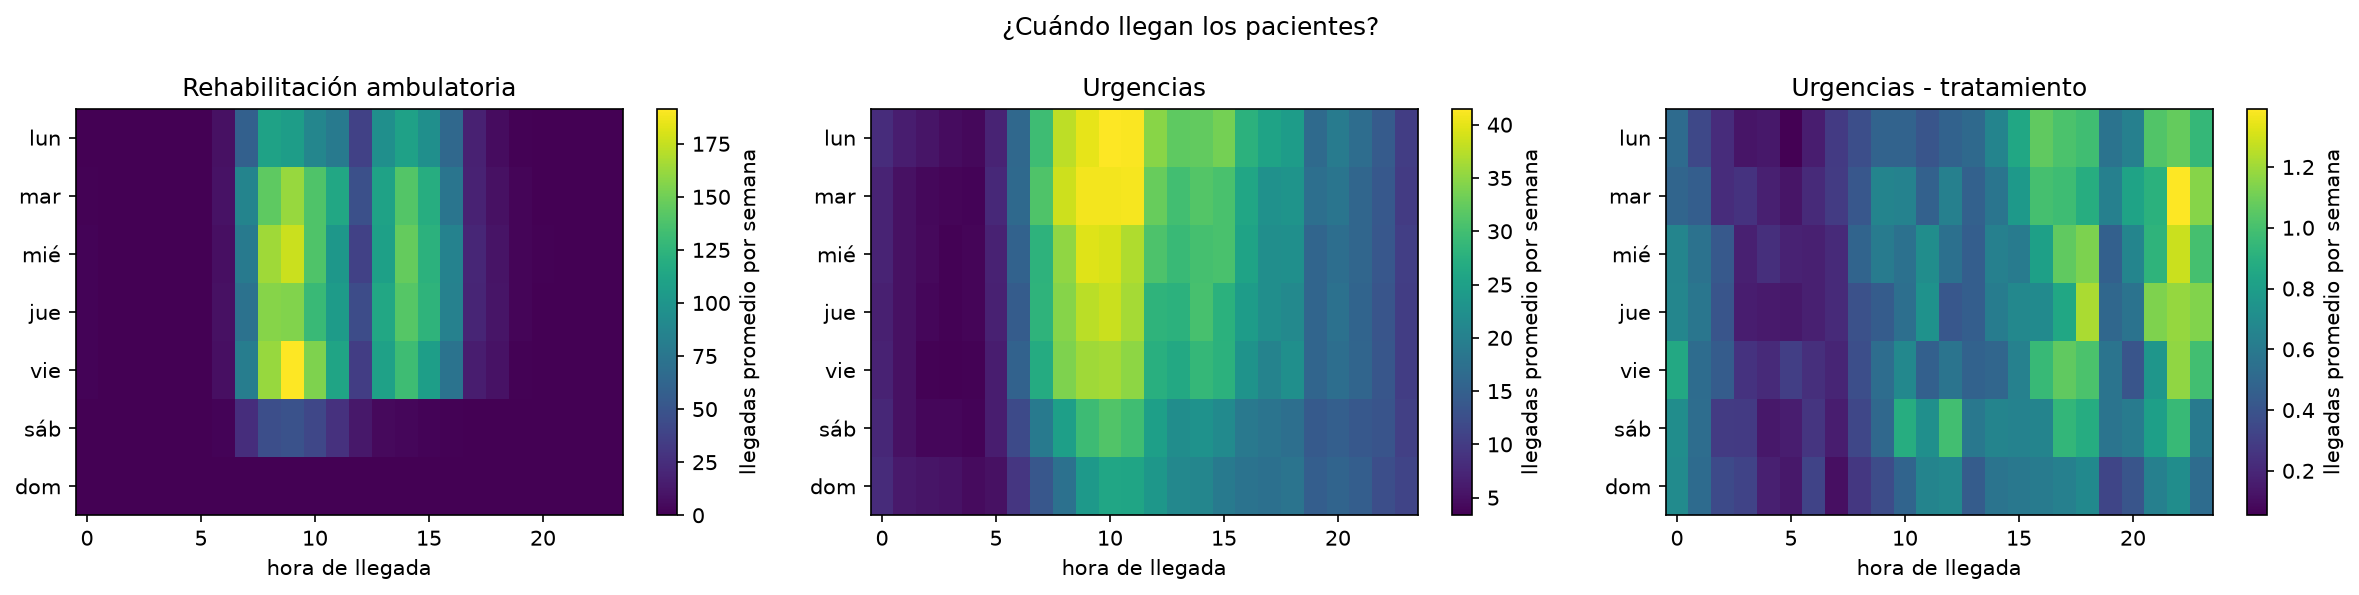
\includegraphics[width=\textwidth]{01_llegadas_dia_hora.png}
\apanota{Figura exploratoria archivada (\texttt{reports/figures/exploracion/01\_llegadas\_dia\_hora.png}). Refleja distribución descriptiva histórica por servicio; no representa una curva de rendimiento predictivo ni debe utilizarse para estimar cifras exactas por lectura visual.}
\end{figure}

\begin{figure}[htbp]
\caption{Tendencia histórica de llegadas diarias en media móvil de 28 días (2023--2026)}
\label{fig:exploracion_tendencia}
\centering
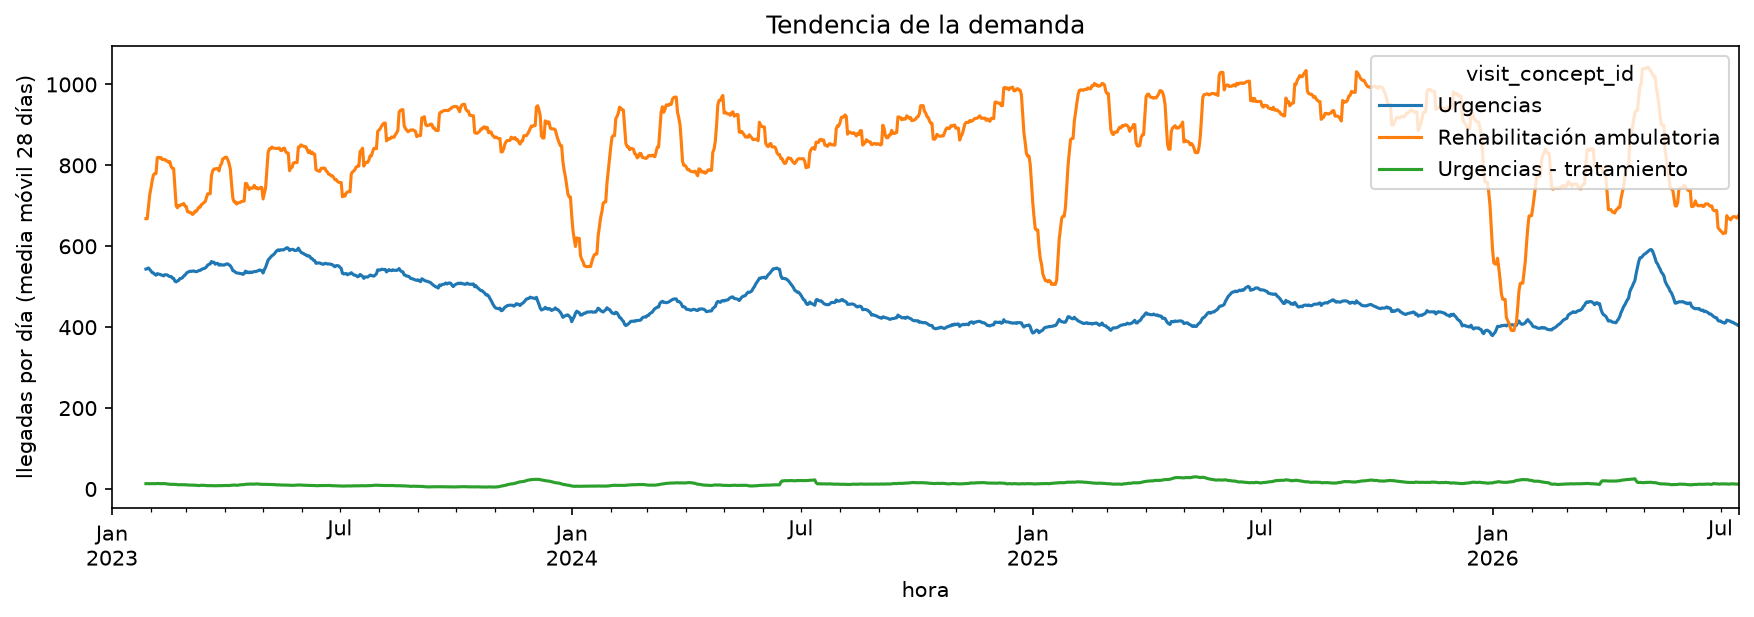
\includegraphics[width=\textwidth]{02_tendencia.png}
\apanota{Figura exploratoria archivada (\texttt{reports/figures/exploracion/02\_tendencia.png}). Muestra la evolución histórica agregada de llegadas y los descensos estacionales de Rehabilitación en Carnaval y cierre de año. No incorpora proyecciones fuera de muestra.}
\end{figure}

\begin{figure}[htbp]
\caption{Duración mediana ($p_{50}$) de etapas según día de la semana y hora de inicio}
\label{fig:exploracion_duracion}
\centering
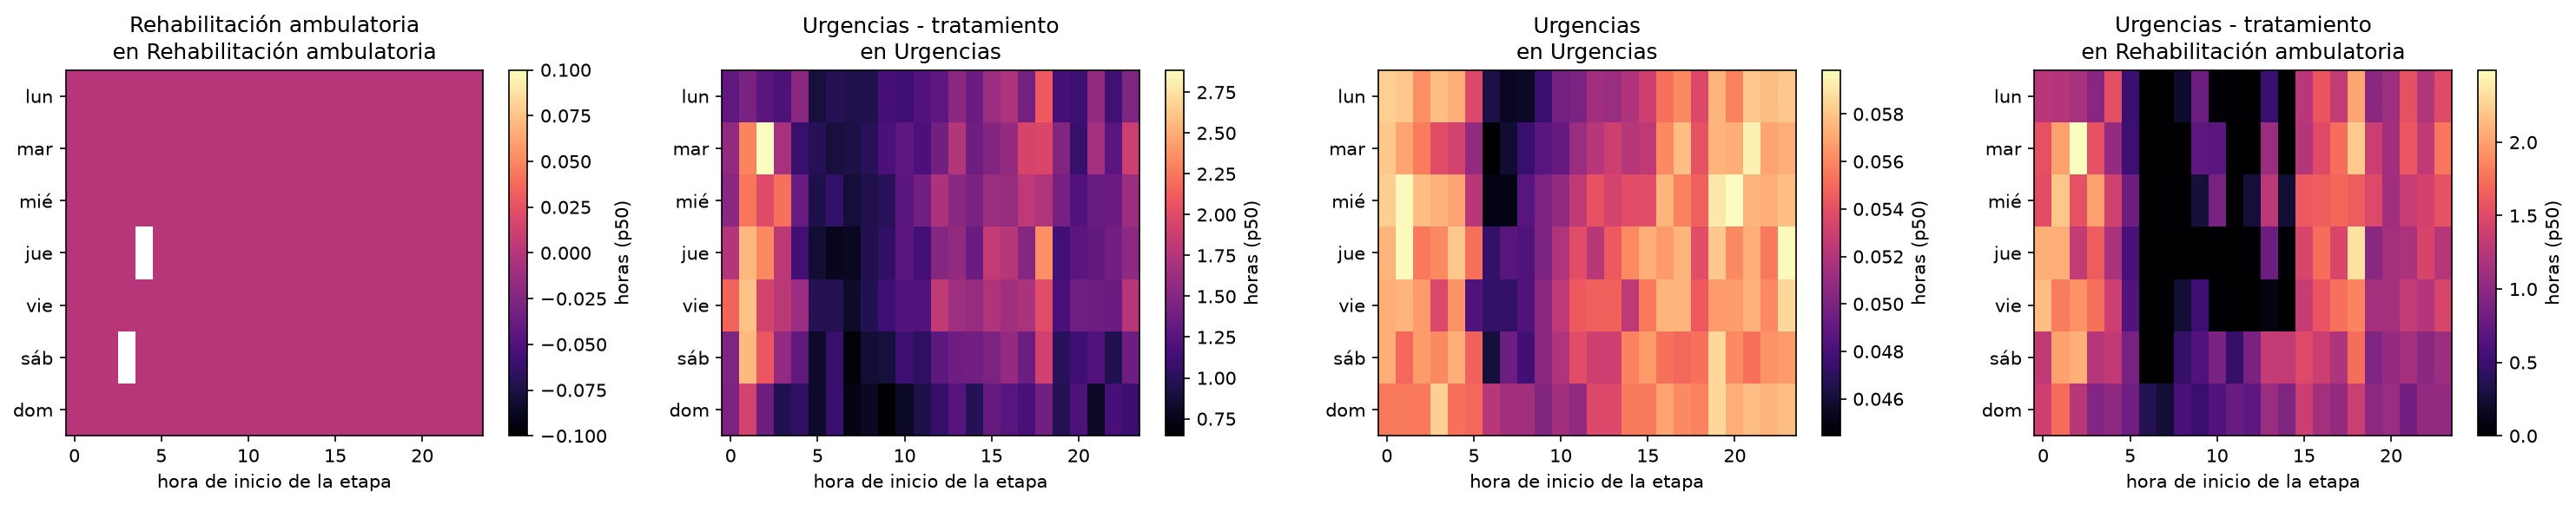
\includegraphics[width=\textwidth]{03_duracion_etapas_franja.png}
\apanota{Figura exploratoria archivada (\texttt{reports/figures/exploracion/03\_duracion\_etapas\_franja.png}). Representa tiempos históricos por franja de inicio en horas; la ausencia de marcas de salida distintas del inicio en Rehabilitación explica los valores nulos en su panel.}
\end{figure}

\subsection{Transición prioritaria entre Tratamiento Urgencias y Hospitalización}

El análisis de pasos secuenciales en \texttt{18\_transiciones\_etapas.sql} identifica como transición prioritaria el salto administrativo desde \textit{Treatment urgency} (\texttt{3045729}) hacia \textit{Inpatient Visit} (\texttt{9201}) dentro de visitas de Urgencias (\texttt{9203}), con \textbf{\num{47670} pasos} acumulados \parencite{mediflow2026optimizacion}. En esta consulta, el indicador de espera entre etapas se define mediante $\text{espera\_h} = \text{inicio\_siguiente} - \text{fin\_anterior}$ sobre etapas con fecha de egreso válida ordenadas por inicio y \texttt{visit\_detail\_id}. En el resumen archivado, el $p_{50}$ mensual ponderado por número de pasos es \num{0,0}\,h y el $p_{90}$ mensual ponderado alcanza \textbf{\num{24,45}\,h} (\num{24,446}\,h sin redondear).

Tres advertencias condicionan la lectura de este indicador. Primero, la definición $\text{inicio\_siguiente} - \text{fin\_anterior}$ admite valores negativos por solapamiento administrativo entre registros, por lo que no equivale a un tiempo clínico de espera por cama asignada ni mide por sí sola episodios de \textit{boarding}. Segundo, el valor \num{24,45}\,h corresponde al promedio de los percentiles $p_{90}$ mensuales ponderado por el volumen mensual de pasos, y no al percentil 90 global calculado sobre los \num{47670} registros individuales agrupados. Tercero, al cruzar mensualmente ese $p_{90}$ con el censo medio mensual de Hospitalización se observa una correlación ecológica negativa de $r = -0{,}481$, con $p_{90}$ ponderado de \num{25,13}\,h en meses de censo normal frente a \num{23,70}\,h en meses de censo alto \parencite{mediflow2026optimizacion}. Este patrón descarta atribuir de forma causal el alargamiento de la transición a la congestión agregada de piso y exige auditar directamente los sellos temporales en el sistema asistencial antes de prometer reducciones de espera por cama mediante redistribución de egresos.
